\par Para realizar un an\'alisis cuantitativo, llamamos $F$ al frame del video real (ideal) que deber\'iamos obtener con nuestro algoritmo, y sea $\bar{F}$ al frame del video efectivamente construido. Consideramos entonces dos medidas, directamente relacionadas entre ellas, como el \emph{Error Cuadr\'atico Medio} (ECM) y \emph{Peak to Signal Noise Ratio} (PSNR), denotados por $\texttt{ECM}(F,\bar{F})$ y $\texttt{PSNR}(F,\bar{F})$, respectivamente, y definidos como:
\begin{equation*}
\texttt{ECM}(F,\bar{F}) = \frac{1}{mn}\sum_{i=1}^m\sum_{j = 1}^n |F_{k_{ij}} - \bar{F}_{k_{ij}}|^2 \label{eq:ecm}
\end{equation*}
\noindent y
\begin{equation*}
\texttt{PSNR}(F,\bar{F}) = 10 \log_{10}\bigg(\frac{255^2}{\texttt{ECM}(F,\bar{F})}\bigg). \label{eq:psnr}
\end{equation*}
\par Ambas métricas se utilizan para medir la diferencia absoluta entre dos señales, en este caso entre los valores de los pixels del video de entrada y del de salida. Los algoritmos implementados para calcular ECM y PSNR calculan dichos valores frame a frame y luego hacen un promedio entre todos los frames del video. Utilizaremos estos promedios obtenidos para comparar la efectividad (en términos cuantitativos) de cada algoritmo, dependiendo de los parámetros de entrada. (El algoritmo para ECM puede encontrarse en el Apéndice \ref{ecmalgo}). 
\par Notar que en los casos en que el ECM entre dos frames sea 0, (debido a que dicho frame no se modificó), el PSNR da infinito. Para calcular el promedio del PSNR de un video, en estos casos, no se tomarán en cuenta dichos frames.

\subsubsection{Experimentación con ECM y PSNR}

\par Para calcular el ECM obtenido a partir de los videos generados con los algoritmos propuestos, implementamos tests que comparan frame a frame el video original ya en slow motion, con el video obtenido luego de eliminar frames intermedios y aplicar cada método para regenerar dichos frames. Es decir, si al video original le eliminamos 2 frames intermedios (utilizando la función \texttt{eliminarFrames}, ver Apéndice \ref{eliminarframes}), compararemos el video original con el video obtenido luego de aplicar cada uno de los algoritmos, tomando como parámetro la misma cantidad de frames intermedios que le habíamos eliminado al video en un principio, en este caso 2.
\par Realizaremos esto para 6 videos diferentes, con distintas calidades y duraciones. Los videos elegidos como inputs se encuentran en slow motion originalmente, y muestran situaciones que consideramos interesantes para analizar resultados cuantitativos y cualitativos, como por ejemplo, una pelota de tenis volando o fideos cayendo lentamente, ya que se pueden apreciar las diferencias con los videos originales más claramente. Además, analizaremos los resultados según el tamaño y calidad del video, ya que algunos algoritmos podrían mejorar su rendimiento en dichos casos. Creemos que videos de mayor calidad generan resultados de mayor precisión.
\par Los tests que generamos calculan el ECM para dichos inputs variando la cantidad de framesIntermedios eliminados al original (2, 4 o 6 frames) para cada algoritmo. Para el algoritmo de splines, a su vez, realiza el mismo cálculo tomando distintos tamaños de bloque (4, 8 o 16 frames por bloque). Con esto pretendemos observar cómo afectan estos parámetros cuantitativamente al resultado final. Bloques de splines de menor tamaño supondrían una mayor precisión debido a que los videos cambian de tomas rápidamente, y al prolongar el tamaño del bloque permite interpolar frames tomando como parámetros frames pertenecientes a distintas tomas, y por lo tanto generar resultados no deseados como imágenes transparentes entre una toma y otra. Estos \textit{artifacts} serán analizados con más detalle en la próxima sección de análisis cualitativo. Aquí nos limitaremos a analizar los resultados cuantitativos.
\par A continuación una breve descripción de los videos de entrada que utilizamos para los tests: (de menor a mayor calidad)
\begin{itemize}
\item \textit{cupcake} : $\#$frames = 252, tamaño 240x360
\item \textit{perro} : $\#$frames = 252, tamaño 360x360
\item \textit{morocho} : $\#$frames = 452, tamaño 360x360
\item \textit{tenis} : $\#$frames = 450, tamaño 240x426
\item \textit{bebes} : $\#$frames = 225, tamaño 544x1280
\item \textit{fideos} : $\#$frames = 125, tamaño 720x1280
\end{itemize}

\par  \textbf{En el Apéndice \ref{cuant} se puede encontrar una tabla con todos los valores obtenidos sobre el ECM promedio y los ECM máximos obtenidos por cada algoritmo para cada input. A continuación estudiaremos el comportamiento de cada método desde distintos enfoques.}

\subsubsection{Resultados sobre ECM y PSNR}

\subsubsubsection{Experimento 1: Efectividad de los métodos según ECM}

\par Comparamos la efectividad de los métodos según el ECM promedio obtenido en cada uno de los inputs con 2 frames intermedios eliminados. Cuanto menor sea el error, consideraremos que el método es más efectivo cuantitativamente. Dejaremos afuera el input \textit{perro} para que el gráfico de barras sea más claro, ya que son valores muy altos comparados a los demás.

\begin{figure}[ht]
	\begin{center}
		\subfigure [Efectividad de los métodos según ECM] {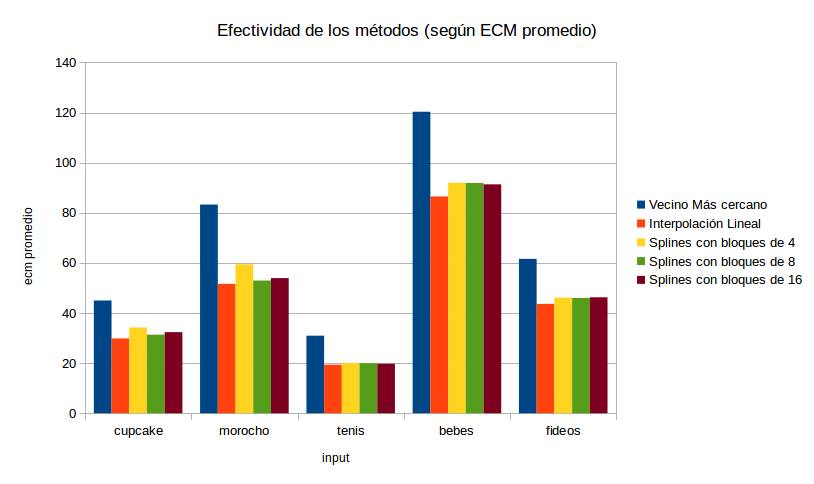
\includegraphics[width=0.9\columnwidth]{imagenes/cuantitativos/exp1.jpg}}
	\end{center}
\end{figure}

\par Se puede observar en el gráfico que el método que arroja mejores resultados con respecto al error cuadrático medio es el de Interpolación Lineal, a diferencia de lo que creíamos. Supusimos que splines por el mayor grado de complejidad de los cálculos y del polinomio interpolante daría como resultado videos más aproximados al original (ideal). Sucede que el algoritmo de splines divide los frames en bloques de como mínimo 4 frames para poder calcular el polinomio de grado 3 (4 variables), lo que hace que en varios de esos bloques los frames pertenezcan a tomas diferentes del video. Si los frames son de tomas diferentes, o los frames varían demasiado entre uno y otro, la función interpolante resultante tiene más error. Como el método lineal "divide" los frames en bloques de a 2, ya que realiza una función cada 2 frames, el impacto de este fenómeno es menor.
\par Además, se puede observar en el gráfico el impacto del \textbf{tamaño de bloque }tomado para realizar los splines. Variar el tamaño del bloque no modifica significativamente el error cometido, sin embargo, estimamos que al aumentar considerablemente el tamaño de los bloques se podrán observar errores visuales (más sobre esto en la sección Análisis Cualitativo).
\par Se puede observar que el tamaño de los videos y la calidad no impacta significativamente en el error cuadrático medio. Sin embargo, el video \textit{perro}  tiene mayores valores de error en todos los algoritmos (ver Apéndice), debido a que es el único de los videos que fue grabado con un celular en movimiento.
\par Por último, variar la calidad del video no trae grandes diferencias en términos cuantitativos, sin embargo, al observar los outputs, se nota una leve mejora del método de splines en términos cualitativos (se producen menos exploits). 

\subsubsubsection{Experimento 2: Impacto del parámetro Frames Internos eliminados}

\par Usando los mismos inputs, correremos los métodos tomando distintas cantidades de frames internos eliminados y compararemos los resultados. Aumentar la cantidad de frames internos a regenerar, debería aumentar el error cuadrático medio.

\begin{figure}[ht]
	\begin{center}
		\subfigure [Efectividad de los métodos según frames intermedios eliminados] {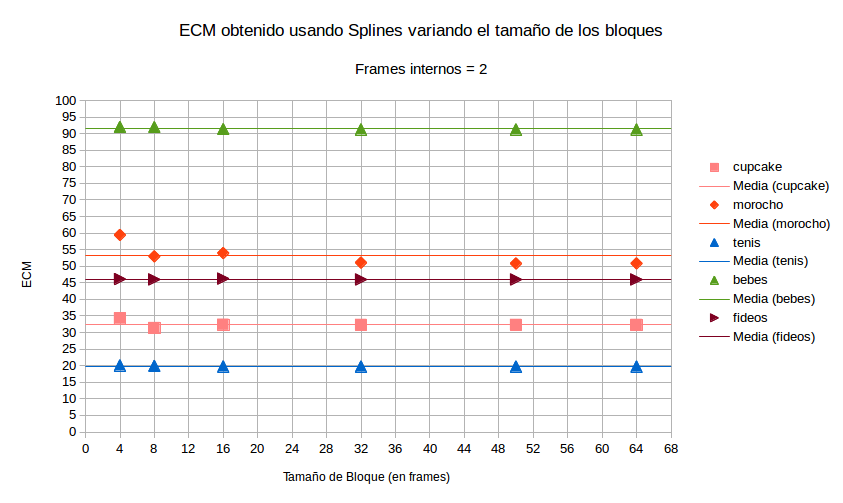
\includegraphics[width=0.9\columnwidth]{imagenes/cuantitativos/exp2.png}}
	\end{center}
\end{figure}

\par En el gráfico se muestran los valores obtenidos al calcular el promedio de los ECM de cada input generados por cada método, según cuál fue la cantidad de frames internos pasada por parámetro.
\par Efectivamente, aumentar framesIntermedios aumenta el error cuadrático medio. Se puede ver en el gráfico que lo hace linealmente, en todos los métodos. Esto se debe a que es mayor la cantidad de frames que se obtienen usando las funciones interpolantes, aumentando el error producido.

\subsubsubsection{Experimento 3: Efectividad de los métodos según PSNR}

\par El PSNR es la métrica utilizada con mayor frecuencia como medida de la calidad objetiva de video. Sin embargo, a causa del comportamiento nolineal del sistema visual humano los valores de PSNR no poseen una perfecta correlación con la calidad visual percibida. 
\par Análogamente, calculamos los PSNR promedio obtenidos con cada algoritmo para los mismos inputs mencionados anteriormente:

\begin{figure}[ht]
	\begin{center}
		\subfigure [Efectividad de los métodos según PSNR] {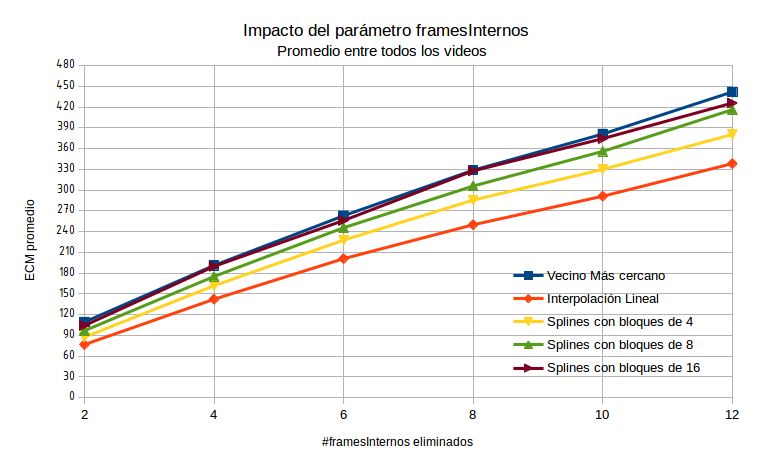
\includegraphics[width=0.9\columnwidth]{imagenes/cuantitativos/exp3.png}}
	\end{center}
\end{figure}

\bigskip

\newpage

\par Como era de esperar, los resultados se corresponden con los obtenidos a partir de comparar los ECM producidos por cada algoritmo. Por definición de PSNR, cuanto menor sea el error, mayor será el PSNR y por lo tanto mejor la calidad.
\par  Interpolación lineal es el método con mayor efectividad en términos cuantitativos.

%\subsubsection{Experimento 4: Usando números fraccionarios vs. enteros para calcular los frames Intermedios}
%
%\par Al momento de implementar el algoritmo de interpolación por splines, nos planteamos dos posibilidades para tomar los valores de los $[x_i]$ (frames del algoritmo). Se podría tener en cuenta los frames Intermedios que necesitamos regenerar o no. Es decir, por ejemplo, teniendo un video de 2 frames, y sabiendo que vamos a agregar 1 frame intermedio (es un caso hipotético, ya que con splines el mínimo es 4 frames), podríamos tener $x_0$ = 0, $x_1$ = 1 y calcular el frame intermedio tomando $x=\frac{1}{2}$ en la función interpolante; o tomar $x_0$ = 0, $x_1$ = 2 y usar $x=1$ para el frame intermedio. En otras palabras, podríamos tomar $h=1$ o $h=framesIntermedios+1$. ($h = x_{i+1} - x_i$)
%\par Este experimento tiene el objetivo de comparar los errores cuadráticos medios producidos por los 3 métodos, implementando ambas opciones, para comprobar nuestra hipótesis sobre que el error se reduce usando números enteros para los frames Intermedios.
%\par El siguiente gráfico muestra los resultados obtenidos al calcular el promedio de los ECM obtenidos para los mismos 6 inputs mencionados anteriormente:
%
%...


